% !TEX root = ../vr_st.tex

\subsection{Spheres and their wedge sum }\label{ss:Sn}\label{subsub:critical values of Sn}

For any integer $n \geq 1$ and real number $\rho > 0$, let $\bS^n(\rho)$ be the \defn{$n$-sphere} of radius $\rho$ centered at the origin of $\R^{n+1}$.
We consider it equipped with the geodesic distance and simplify notation writing \(\bS^n\) instead of \(\bS^n(1)\).

%We apply the notations and results from \cref{sub:general_barcodes} to the Vietoris--Rips complexes of $\bS^n$ with $R = \pi$ the diameter of the sphere.
%Let \(\degp \in \N\) and \(\theta \in \cO(\ell,\degp)\) a linear cohomology operation with \(\ell \neq \degp\).

\medskip\proposition
% Let $\crit(\bS^n), \firstdeath{m}{\bS^n}$ and $\firstdeath{\theta}{\bS^n}$ be respectively the first critical values of $\VR(\bS^n)$, its $\degp^{\th}$ reduced homology, and its $\img_\theta$-module for some \(\theta \in \cO(\ell,\degp)\) with \(\ell \neq \degp\).
% Then:
For any integer $m \in \N$ and $\theta \in \cO(\ell, m)$:
\[
\mathrm{(1)}\ \crit(\bS^n) = \zeta_n,
\qquad
\mathrm{(2)}\ \firstdeath{m}{\bS^n} =
\begin{cases}
	\zeta_n & m = n, \\
	\hfil 0 & m \neq n,
\end{cases}
\qquad
\mathrm{(3)}\ \firstdeath{\theta}{\bS^n} = 0,
\]
where \(\zeta_n = 2 \cdot \fillrad(\bS^n)\).
%= \arccos(\tfrac{-1}{n+1})\).

\begin{proof}
	(1) Recall from \cite[Thm.~7.1]{lim2020vietoris} that for any $0 < r \leq \zeta_n$, the space $\VR_r(\bS^n)$ is homotopy equivalent to $\bS^n$, and the homotopy type of $\VR_r(\bS^n)$ changes at $\zeta_n$.
%	\footnote{
%		The case $n = 1$ has more information.
%		From \cite[Thm.~7.4]{adamaszek2017vietoris} it is known that $\VR_r(\bS^1)$ is homotopy equivalent to $\bS^{2n+1}$ for any $n \in \N$ and $\frac{2n\pi}{2n+1} < r \leq \frac{2(n+1)\pi}{2n+3}$.
%		For $d=1$ and $n > 1$ and one also has more information.
%		Recall that a metric space $(\cX, d)$ is said to be a \defn{geodesic space} if for each $x, y \in \cX$ there exists geodesic from $x$ to $y$ of length $d(x, y)$.
%		As stated in \cite[Prop.~7.10]{virk20201} one knows that if $\cX$ be a simply-connected geodesic space, then $\barc\rH_1(\cX) = \emptyset$.
%		Since the spheres we are considering are geodesic their $\rH_1$ barcode is empty.}
	This implies $\crit(\bS^n)=\zeta_n$.

	(2) According to \cite{katz1983filling}, \(\mathrm{FillRad}(\bS^n) = \frac{1}{2}\zeta_n\).
	From \cref{ss:filling_radius}, it follows that \((0, \zeta_n)\) is a bar in the \(n^{\text{th}}\) reduced homology of \(\VR (\bS^n)\).
	Thus, \(\crit_n(\bS^n) \leq \zeta_n\).
	On the other hand, we have \(\crit_n(\bS^n) \geq \crit(\bS^n) = \zeta_n\).
    Thus, we conclude that \(\crit_n(\bS^n) = \zeta_n\).
    When $m\neq n$, the statement follows from the fact that the initial space in the filtration has trivial $\degp^{\th}$ reduced homology.

	(3) We apply a similar argument as in the $m\neq n$ case of (2). The statement follows from the fact that the initial space in the filtration has trivial $\img_\theta$ for any \(\theta \in \cO(\ell,\degp)\) with \(\ell \neq \degp\). 
	% \footnote{The fact that for $0 < r < \zeta_n$ the spaces $\VR_r(\bS^n)$ and $\bS^n$ are homotopy equivalent was shown in \cite[Theorem 7.1]{lim2020vietoris} using the filtered homotopy equivalence between the Vietoris-Rips filtration and the Kuratowski filtration. Our claim is that $f_r^n$ is a weak equivalence.\anibal{This comment is redundant given that the first critical value of is \(\zeta_n\).}}
\end{proof}

\subsubsection{}\label{ss:VRSn projection}

From the previous proposition we know that for \(r \in (0, \zeta_n)\) the spaces \(\VR_r(\bS^n)\) and \(\bS^n\) have the same homotopy type for any \(n \in \N\).
We now recall from \cite{adamaszek2020homotopy} a natural map realizing this equivalence.

For \(n \in \N\) and \(r < \pi\) \ling{change to $\zeta_n$}, the \defn{\(\VR_r(\bS^n)\)-projection}
\[
f_r^n \colon \VR_r(\bS^n) \to \R^{n+1} \setminus \set{0} \to \bS^n
\]
is the composition of the map sending a formal linear combination $\sum\lambda_i x_i$ to the point \(\sum\lambda_i x_i\) in \(\bbR^{n+1}\) and the map sending a point in \(\R^{n+1} \setminus \set{0}\) to its radial projection.\anibal{I would like a comment about why this is well defined. \ling{done.}}
The well-definedness of $f_r^n$ follows from a similar argument to that in \cite[Lemma 3]{lovasz1983self}, where the original proof is for Euclidean spheres, but a similar proof applies for geodesic spheres. 
%The main idea in the proof is that if the polytope formed by $\{x_i\}$ contains the origin, then the diameter of $\{x_i\}$ exceeds $\zeta_n$

\medskip\proposition
The \(\VR_r(\bS^n)\)-projection is a homotopy equivalence when $r \in (0, \zeta_n)$.

\begin{proof}
    \anibal{in [18] a new topology was introduce on VR and the authors show that, whith respect to this topology the projection is a homotopy equivalence. More recently, gill showed that the identity map is a weak equiv from VR with its CW topology to the other. Therefore, the projection is a weak equivalence from the usual VR, and therefore, since CW spaces, a homotopy equivalence.}

	To prove the statement, we use an intermediate construction called the Vietoris--Rips thickening, introduced in \cite{adamaszek2018metric} as a metric space analogue of the Vietoris--Rips complexes.

	The Vietoris--Rips thickening $\VR_r^m\cX$ of a metric space $\cX$ at a given scale $r$ is defined as the set of convex linear combinations of the Dirac probability measures $\delta_{x}$ on points $x \in X$, equipped with the $1$-Wasserstein metric.
	There is a set bijection from $g_r \colon \VR_r\cX \to \VR_r^m\cX$, given by $\sum \lambda_i x_i \mapsto \sum \lambda_i \delta_{x_i}.$
	%As this object is not the center of the discussion here, we omit the details and only state the related results here.
	It is shown in \cite[Theorem 1]{gillespie2024vietoris} that the natural bijection $g_r$ is a weak homotopy equivalence.

	In the case of $\cX = \bS^n$, the map $f_r^n$ is the composition of two maps
	\[
	\VR_r(\bS^n) \xrightarrow{g_r} \VR_r^m(\bS^n) \xrightarrow{f_r^n \circ g_r^{-1}} \bS^n.
 	\]
	According to \cite[Proposition 5.3]{adamaszek2018metric}, when $0<r<\zeta_n$, $f_r^n \circ g_r^{-1}$ is a homotopy equivalence, implying that $f_r^n = (f_r^n \circ g_r^{-1}) \circ g_r$ is a weak homotopy equivalence.
\end{proof}

\subsubsection{}

\label{subsub:barcode_Sn}

We apply the above proposition \ling{explain how} and the barcode estimates from \cref{sub:general_barcodes} to \(\bS^n\), by taking \(R = \diam(\bS^n) = \pi\).
Using the facts (1) that the reduced homology of \(\bS^n\) has dimension one for \(m = n\) and is zero for all other values of \(m\), and (2) that for any linear cohomology operation \(\theta \in \cO(\ell, m)\) with \(\ell \neq m\), \(\img \theta_{\bS^n}\) is trivial, we proceed with the estimation but omit the figure, as it is simply a special case of \cref{fig:barcodes_vs}.

\ling{use reduced homology and reference to other results; improve the paragraph.}


% \begin{figure}[ht]
% 		\centering
% 		\begin{tabular}{ c c }
	\begin{tikzpicture}[scale=0.6]
		\begin{axis} [
			title = {\LARGE $\barc\rH_n(\bS^n)$},
			ticklabel style = {font=\Large},
			axis y line=middle,
			axis x line=middle,
			ytick={0.5,0.57,0.67,0.95},
			yticklabels={,$\zeta_n$,,$\pi$},
			xtick={0.5,0.57,0.95},
			xticklabels={$\frac{\pi}{2}$,$\zeta_n$, $\pi$},
			xmin=-0.015, xmax=1.1,
			ymin=0, ymax=1.1,]
			\addplot [thick,color=black!20!white,fill=black!30!white,
			fill opacity=0.4]coordinates {
				(0.57,0.95)
				(0.57,0.57)
				(0.95,0.95)
				(0.57,0.95)};
			\addplot [black!40!white,mark=none,dashed, thin] coordinates {(0,0.57) (0.57,0.57)};
			\addplot [black!40!white,mark=none,dashed, thin] coordinates {(0.57,0) (0.57,0.57)};
			\addplot[barccolor,mark=*] (0, 0.57) circle (2pt) node[above right,barccolor]{};{\Large\textsf{1}};
			\addplot [mark=none] coordinates {(0,0) (1,1)};
		\end{axis}
	\end{tikzpicture}
	&
	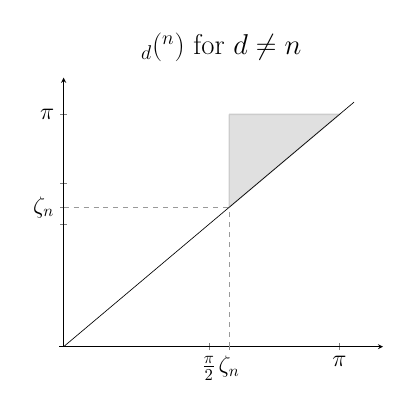
\begin{tikzpicture}[scale=0.6]
		\begin{axis} [
			title = {\LARGE $\barc\rH_d(\bS^n)$ for $d \neq n$},
			ticklabel style = {font=\Large},
			axis y line=middle,
			axis x line=middle,
			ytick={0.5,0.57,0.67,0.95},
			yticklabels={,$\zeta_n$,,$\pi$},
			xtick={0.5,0.57,0.95},
			xticklabels={$\frac{\pi}{2}$,$\zeta_n$, $\pi$},
			xmin=-0.015, xmax=1.1,
			ymin=0, ymax=1.1,]
			\addplot [thick,color=black!20!white,fill=black!30!white,
			fill opacity=0.4]coordinates {
				(0.57,0.95)
				(0.57,0.57)
				(0.95,0.95)
				(0.57,0.95)};
			\addplot [black!40!white,mark=none,dashed, thin] coordinates {(0,0.57) (0.57,0.57)};
			\addplot [black!40!white,mark=none,dashed, thin] coordinates {(0.57,0) (0.57,0.57)};
			\addplot [mark=none] coordinates {(0,0) (1,1)};
		\end{axis}
	\end{tikzpicture}
\end{tabular}
% 		\caption{Persistent homology barcode of $\bS^n$. The right-hand-side figure
% 		\emph{Right:} $\theta$-barcodes of $\VS$ where $\theta \in \cO(\ell,m)$ is any linear cohomology operation with \(\ell \neq m\).
%         In each figure, the gray region represents where additional bars could exist within the corresponding barcode.
% 		We remark that for any \(n \in \N\) the value \(\zeta_n\) is bounded below by \(\pi/2\).}
% 		\label{fig:Sk}
% 	\end{figure}

\subsubsection{}

For $n \in \N$ and $\ell_1, \dots, \ell_n \in \N^n$, let
\[
\VS^{\ell_1,\dots,\ell_n} =
\overbrace{\bS^1\vee\dots\vee\bS^1}^{\ell_1} \vee\dots\vee \overbrace{\bS^n\vee\dots\vee\bS^n}^{\ell_n}.
%(\bS^1)^{\vee m_1} \vee \dots \vee (\bS^n)^{\vee m_n}.
\]
Using the homotopy equivalence between the Vietoris--Rips filtration of a metric gluing with the wedge sum of the Vietoris--Rips filtration described in \cref{ss:wedge sum}, we have the following isomorphisms of persistence modules for \(\degp \in \N\) and \(\theta \in \cO(\ell,\degp)\):
\[
\begin{split}
	\rH_\degp (\VR\VS^{\ell_1,\dots,\ell_n}) &\cong \, \bigoplus_{i=1}^n \rH_\degp (\VR\bS^i)^{\oplus \ell_i}, \\
	\img_\theta \VR(\VS^{\ell_1,\dots,\ell_n}) &\cong \, \bigoplus_{i=1}^n (\img_\theta \VR\bS^i)^{\oplus \ell_i}.
\end{split}
\]

Therefore, both the homology barcodes and \(\img_\theta\)-barcodes of \(\VS^{\ell_1, \dots, \ell_n}\) are the multiset unions of the corresponding barcodes of \(\bS^1, \dots, \bS^n\); see \cref{fig:barcodes_vs}.

% $\rH_\degp(\VS^{\ell_1,\dots,\ell_n})$ contains $\ell_\degp$ copies of $(0,\zeta_\degp)$.
% All remaining bars in this barcode must be dominated by $(\zeta_n, \pi)$.
% This holds for all degrees, with the convention that $\ell_\degp = 0$ for $\degp > n$.

% Similarly, for any linear cohomology operation $\theta \in \cO(\ell,m)$ with $\ell \neq m$, every bar in either its $\img\theta$ or $\ker\theta$ barcode is dominated by $(\zeta_n, \pi)$.

\begin{figure}
	\centering
	\begin{tikzpicture}[scale=0.52]
	\begin{axis} [
		title = {\LARGE $\Hbarc[\field]{\degp}{\VS^n},1\leq \degp\leq n$},
		ticklabel style = {font=\Large},
		axis y line=middle,
		axis x line=middle,
		ytick={0.5,0.6,0.67,0.95},
		yticklabels={,$\zeta_\degp$,,$\pi$},
		xtick={0.5,0.55,0.95},
		xticklabels={$\frac{\pi}{2}$,$\zeta_n$, $\pi$},
		xmin=-0.015, xmax=1.1,
		ymin=0, ymax=1.1,]
		\addplot [mark=none] coordinates {(0,0) (1,1)};
		\addplot [thick,color=black!20!white,fill=black!30!white,
		fill opacity=0.4]coordinates {
			(0.55,0.95)
			(0.55,0.55)
			(0.95,0.95)
			(0.55,0.95)};
		\addplot [black!40!white,mark=none,dashed, thin] coordinates {(0,0.6) (0.6,0.6)};
		\addplot [black!40!white,mark=none,dashed, thin] coordinates {(0,0.55) (0.55,0.55)};
		\addplot [black!40!white,mark=none,dashed, thin] coordinates {(0.55,0) (0.55,0.55)};
		\addplot[barccolor,mark=*] (0, 0.6) circle (2pt) node[above right,barccolor]{};%{\Large\textsf{1}};
		%\node[mark=none] at (axis cs:0.68,0.21){$\Hbarc{2}{\VS^n}$};
	\end{axis}
\end{tikzpicture}
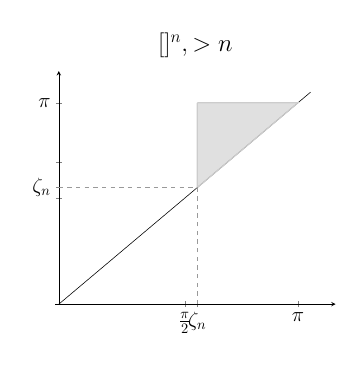
\begin{tikzpicture}[scale=0.52]
	\begin{axis} [
		title = {\LARGE $\Hbarc[\field]{\degp}{\VS^n}, \degp>n$},
		ticklabel style = {font=\Large},
		axis y line=middle,
		axis x line=middle,
		ytick={0.5,0.55,0.67,0.95},
		yticklabels={,$\zeta_n$,,$\pi$},
		xtick={0.5,0.55,0.95},
		xticklabels={$\frac{\pi}{2}$,$\zeta_n$, $\pi$},
		xmin=-0.015, xmax=1.1,
		ymin=0, ymax=1.1,]
		\addplot [mark=none] coordinates {(0,0) (1,1)};
		\addplot [thick,color=black!20!white,fill=black!30!white,
		fill opacity=0.4]coordinates {
			(0.55,0.95)
			(0.55,0.55)
			(0.95,0.95)
			(0.55,0.95)};
		\addplot [black!40!white,mark=none,dashed, thin] coordinates {(0,0.55) (0.55,0.55)};
		\addplot [black!40!white,mark=none,dashed, thin] coordinates {(0.55,0) (0.55,0.55)};
		%\node[mark=none] at (axis cs:0.68,0.21){$\Hbarc[\field]{\degp}{\VS^n}, \degp\geq 3$};
	\end{axis}
\end{tikzpicture}

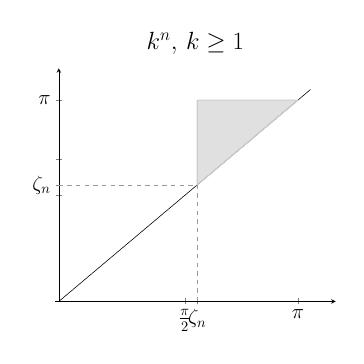
\begin{tikzpicture}[scale=0.52]
	\begin{axis} [
		title={\LARGE $\sqbarc{k}{\VS^n},\, k\geq 1$},
		ticklabel style = {font=\Large},
		axis y line=middle,
		axis x line=middle,
		ytick={0.5,0.55,0.67,0.95},
		yticklabels={,$\zeta_n$,,$\pi$},
		xtick={0.5,0.55,0.95},
		xticklabels={$\frac{\pi}{2}$,$\zeta_n$, $\pi$},
		xmin=-0.015, xmax=1.1,
		ymin=0, ymax=1.1,]
		\addplot [mark=none] coordinates {(0,0) (1,1)};
		\addplot [thick,color=black!20!white,fill=black!30!white,
		fill opacity=0.4]coordinates {
			(0.55,0.95)
			(0.55,0.55)
			(0.95,0.95)
			(0.55,0.95)};
		\addplot [black!40!white,mark=none,dashed, thin] coordinates {(0,0.55) (0.55,0.55)};
		\addplot [black!40!white,mark=none,dashed, thin] coordinates {(0.55,0) (0.55,0.55)};
		%\node[mark=none] at (axis cs:0.68,0.21){$\sqbarc{k}{\VS^n},\, k\geq 1$};
	\end{axis}
\end{tikzpicture}

	\caption{Let $\VS = \VS^{\ell_1,\dots,\ell_n}$ for some tuple of non-negative integers.
		\emph{Top row:} persistent reduced homology barcodes of $\VS$, where the dot $(0,\zeta_m)$ has multiplicity $\ell_m$ which can be zero.
		\emph{Bottom row:} $\img_\theta$-barcodes of $\VS$ where $\theta \in \cO(\ell,m)$ with \(\ell \neq m\).
        In each figure, the gray region represents where additional bars could exist within the corresponding barcode. \ling{we are using both $\ell$ and $\ell_m$}}
	\label{fig:barcodes_vs}
\end{figure}